\section{Heading Uno}
Lorem ipsum dolor sit amet, consectetur adipiscing elit. Nam ultrices ligula dui, non bibendum urna interdum eu. Duis ipsum lorem, ornare non pellentesque in, feugiat ac risus. In vitae nunc tortor. Donec sapien ex, ultricies vitae lorem et, eleifend ullamcorper metus. Nullam sed bibendum lectus, id mattis nulla.\medskip

\begin{figure}[H]
    \centering
    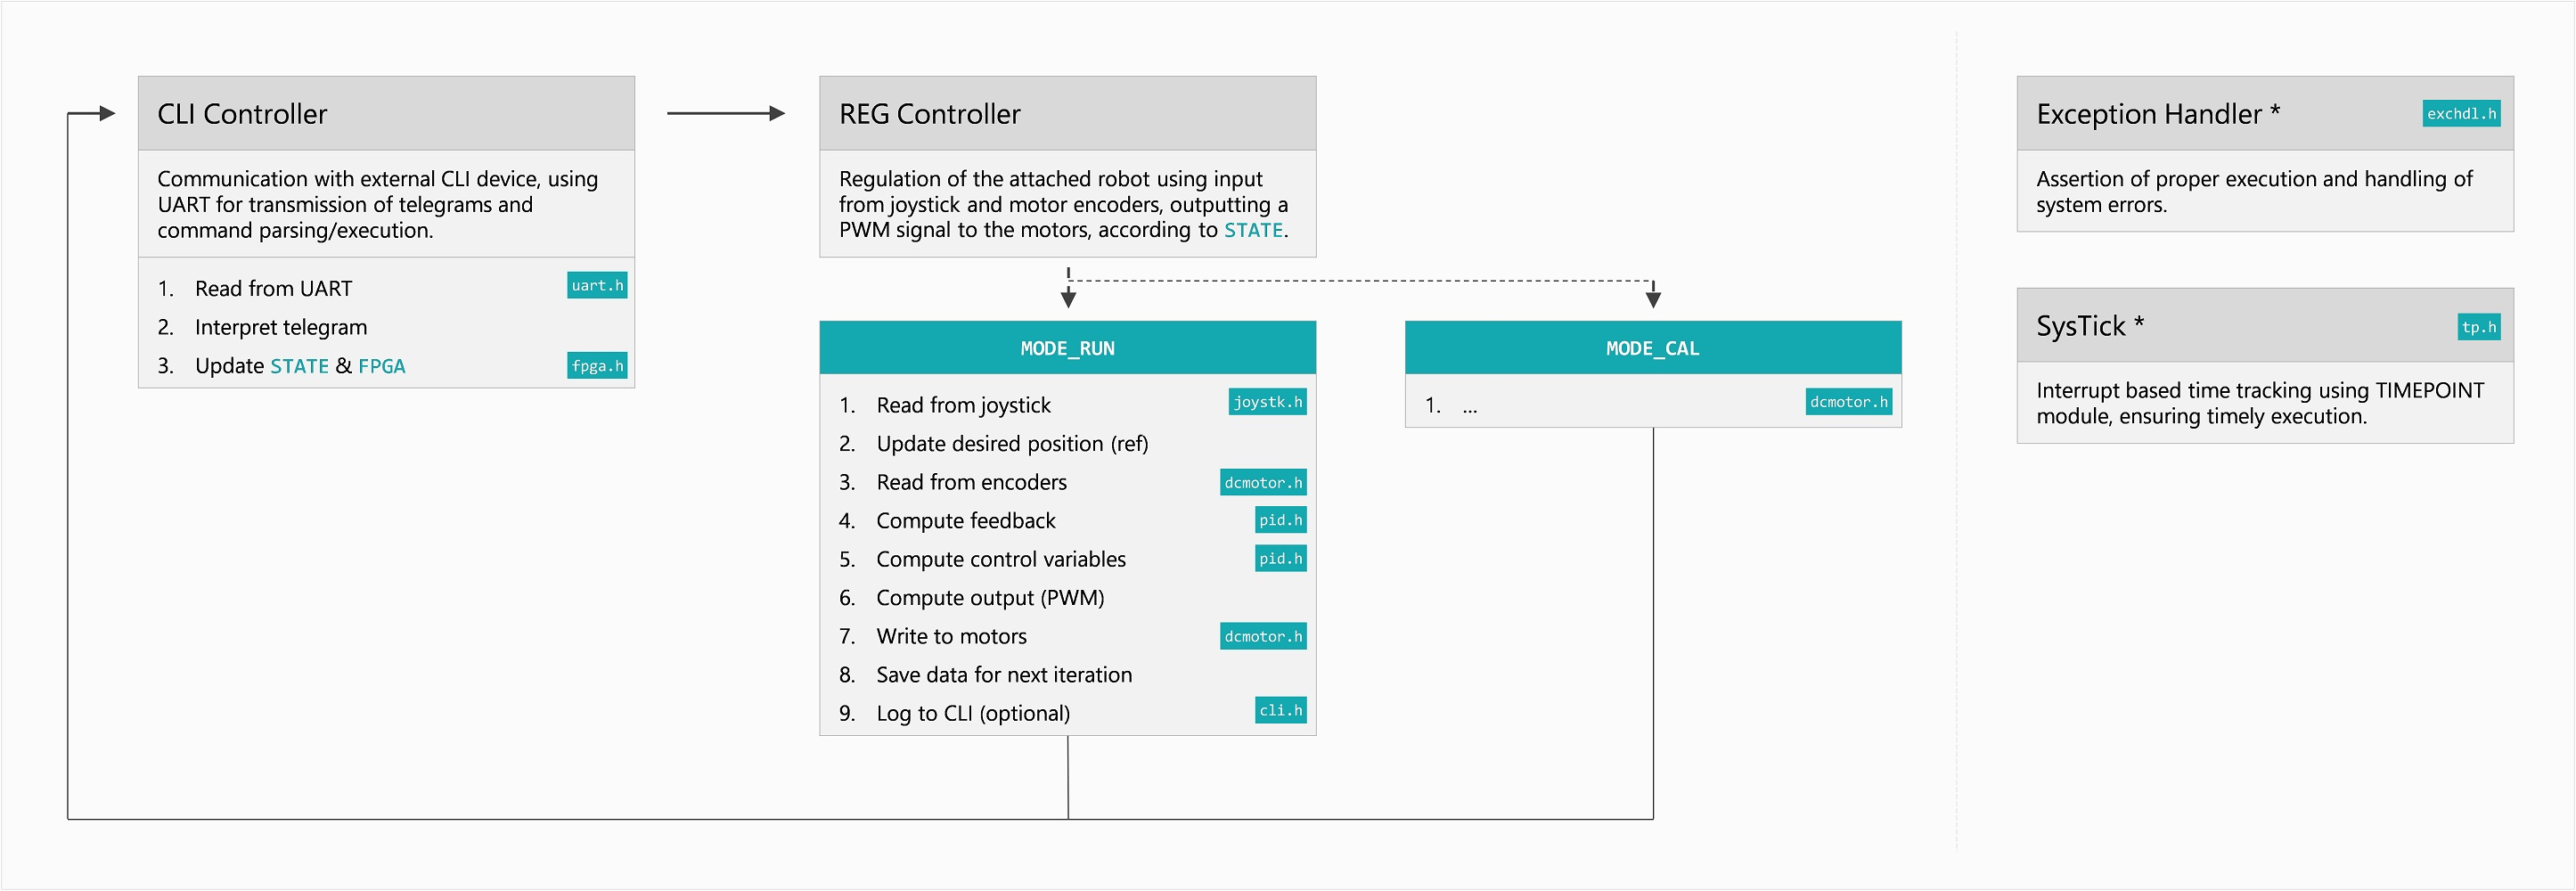
\includegraphics[width=\textwidth]{assets/img/mcu_architecture.jpg}
    \caption{Overview of system architecture.}
    \label{fig:mcu_architecture}
\end{figure}

\section{Heading Dos}
Lorem ipsum dolor sit amet, consectetur adipiscing elit. Nam ultrices ligula dui, non bibendum urna interdum eu. Duis ipsum lorem, ornare non pellentesque in, feugiat ac risus. In vitae nunc tortor. Donec sapien ex, ultricies vitae lorem et, eleifend ullamcorper metus. Nullam sed bibendum lectus, id mattis nulla.\medskip

\newpage
This is a test-code snippet:\medskip

\begin{lstlisting}[language=C]
#include <stdio.h>
#define N 10
/* Block
 * comment */

int main()
{
    int i;

    // Line comment.
    puts("Hello world!");
    
    for (i = 0; i < N; i++)
    {
        puts("LaTeX is also great for programmers!");
    }

    return 0;
}
\end{lstlisting}\medskip

Which is maybe described by this equation?
\begin{equation}
\label{eq:some_eq}
t_{tone} -(2 \cdot a_{fade} \cdot t_{tone}) \geq 2 \cdot t_{chunk} 
\end{equation}

In vitae nunc tortor. Donec sapien ex, ultricies vitae lorem et, eleifend ullamcorper metus. Nullam sed bibendum lectus, id mattis nulla. Maybe equation \ref{eq:some_eq} wasn't so good; how about this neatly aligned enumeration with SI units and mathematical symbols?\medskip

\begin{itemize}[noitemsep]
\NumTabs{2}
    \item Samtidige klienter:
          \tab{$\geq$ 2}
    \item Fejlrate: 
          \tab{$\leq$ 5\%}
    \item Størrelse af payload: 
          \tab{$\geq$ 3 bit} 
    \item Inputrate:
          \tab{$\approx$ \SI{5}{\hertz}} 
\end{itemize}